\documentclass[11pt]{article}
\usepackage[english]{babel}
\usepackage[T1]{fontenc}
\usepackage{amsmath}
\usepackage{amsfonts}
\usepackage{graphicx}
\usepackage{hyperref}
\usepackage{mathtools}
\usepackage{url}
\usepackage[utf8]{inputenc}
\usepackage{caption}
\usepackage{listings}
\usepackage{fullpage}
\usepackage[colorinlistoftodos]{todonotes}
\usepackage[top=0.5 in, bottom =0.5 in, left = 0.5 in, right = 0.5 in ]{geometry}
\newcommand{\R}{\mathbb{R}}
\newcommand{\E}{\mathbb{E}}

% for proof environment and theorem environment (among others)
\usepackage{amsthm}

% for paragraph spacing
\setlength{\parskip}{2pt}%
\setlength{\parindent}{0pt}%


%%%%%%%%%%%%%%%%%%%%%%%%%%%%%%%% GAME PLAN COMMENT %%%%%%%%%%%%%%%%%%%%%%%%%%%%%%
%% Alex will take care of Boston, Luis will take care of San Francisco Crime Data. 

%% These are the steps for fitting linear regression to these models. 
%% 1) Partition the data into something sensible. We will take the data from the cities, and subdivide into regions using the latitude and longitude data for each city. 
%%   1. What we can do for our linear regression model is vary the number of partitions. We will always divide into an nxn grid, and so we have a parameter n. For different values of this parameter (ranging from n = 1 to n = 30 or something, depending on our data models, we will run linear regression on the TIME SERIES data for each sub-region.
%%   2. TIME SERIES linear regression will involve simply regressing on the time as a feature.
%%      - We discretize time based on days (and months) from the earliest date available. Anything we do to the data should be discussed more thoroughly in the data collection and processing section. 
%%      - Another thing to take into account is that we will be normalizing our data. 
%%   3. For testing purposes, we will attempt to hold out data in two way for each region.
%%      a. We hold out data based on year. So, we train on all data from 2001-2012, and then test on the data from 2013.
%%      b. We hold out on data randomly, around 10%. So we train on a random subset of the data from all years, and then we test on the held out data.
%%   4. Figures and plots:
%%      a) For linear regression, we're varying the value of n for the location bucketization. For each region, we calculate the RMSE, and then we can take the average of these RMSEs. Ie, if n = 3, we have 9 linear regressors for each region, and then for each region we can test on our predicted data, giving us an RMSE for that each of the 9 regions. We then just take the average RMSE of the results to take the overall RMSE.
%%  5. We can explore other features, for example, trying to run linear regression on just the entire data set - this includes the time and location data.


%%%%%%%%%%%%%%%%%%%%%%%% INTRUCTIONS FOR ABSTRACT %%%%%%%%%%%%%%%%%%%%%%%%%%%%%%%%%%%%%%%%%%%%%%
% Your Abstract should be short 4-6 sentences that reads like a paper abstract without results (e.g. there should be some motivation + how you tackle the problem).  You will receive points for crafting a succinct summary + professional writing.

% 2. Your Update should include (a) any changes to your proposal, (b) status of data collection and processing [this should be complete!], (c) numbers/graphs showing your baseline.  Theoretical projects should have a literature review relating to your specific question instead of data and baselines.  You may lose points for not implementing course corrections on the proposal (if any were required) and if you are behind on data/baselines without having moved to/explained a back-up plan.

\begin{document}

\title{CS 281 Project Update: Crime Prediction}
\author{Alex Wang  and Luis Perez}
\date{November 2015}

\maketitle

\begin{abstract}
% Make sure we describe our motivation, and the process we take to approach it.
% No need to discuss results yet
% It'd be great if we could get a paper for current approaches; isn't it primarily just using historical averages?
Though average crime rates in the United States have been in the decline for the last few years \cite{seasonal_pattern}, it is still useful to many groups, such as law enforcement, city officials, home buyers, etc., to be able to predict where and when crime will occur. We develop a model to predict future crime incidence at a future time given a geographical location, leveraging historical crime data from the cities of Boston, Chicago, and San Francisco. We take a Bayesian non-parametric approach to the problem of interpolation on crime data from these cities. We explore Gaussian Processes with simple closed form kernels which have proven effective at inferring CO2 levels \cite{gaussian_models}. We compare these models to current baseline approaches which consists of linear regression on crime data, partitioned by region.
\end{abstract}


\section{Proposal Modifications}
% Discuss any changes that you made in direction (a few sentences is fine, as long as it's clear).  Please explicitly note if you've made a major change.
The largest modification between our project now and the proposal consists of dropping the requirement of implementing a neural network or a hidden markov model. Instead, we plan to focus primarily on Gaussian processes, and only considering other models if there is extra time to do so. The main reason for this change is the suggestion made by Finale, as well as the success of analytically solvable GPs in predicting time series data. Therefore, we expect to study variants of the standard covariance kernel for GPs, reporting the results of these models as applied across our three cities. \\

Another major modification to our proposal, and a concern noted in our original feedback, was simplification of the data sources we are drawing together. Previously we had noted that we would harness the full capacity of the open city data movement, by layer information about property values, community center locations, geo-located Tweets, etc. After a more thorough investigation of the data, we found this to be infeasible for many reasons, and we are focusing on the crime data itself. First, the data often was limited to only one year, while our crime data extended back several years, meaning that in order to incorporate other features, we would have to throw away a portion of our most relevant statistic, the crime data itself. Second, the data provided varied widely between cities. Though one city might provide information about property values, another city did not but provided information about police station locations instead. These inconsistencies made it difficult to apply our methods to multiple cities, something we found undesirable.\\

The baseline comparison remains linear regression, and we present those results below. We expect well implemented GPs to outperform the baseline, and GPs which take into account the interrelation between geographical regions to outperform all others.

\section{Data Collection and Processing}
We expect to explore three sets of data, all currently publicly available. These datasets mostly conform to the same standards, so the fields we seek to use are available across all these datasets
\begin{enumerate}
\item \href{https://data.cityofchicago.org/Public-Safety/Crimes-2001-to-present/ijzp-q8t2?q=crime}{City of Chicago Crime Dataset}. The relevant data includes: longitude, latitude, time, date, and type of crime. The set contains a total of approximately 6 million records, dating back to 2001. We remove outliers in any of the above fields form the dataset.
\item \href{https://data.sfgov.org/Public-Safety/Map-Crime-Incidents-from-1-Jan-2003/gxxq-x39z}{San Francisco Crime Mapping}: Again, the relevant data includes: longitude, latitude, time, date, and type of crime. In this data set, we also drop outliers. The total size is 1.8 million crime incidents. 
\item \href{https://data.cityofboston.gov/Public-Safety/Crime-Incident-Reports/7cdf-6fgx}{Boston Crime Incident Reports}: appoximately $250,000$ entries after cleaning, dating back to 2012 to present.
\end{enumerate}

The above data has been processed in a way that allows us to create $n\times n$ time-series over $n \times n$ discrete regions for each geographical city. 
\begin{enumerate}
\item The data is partitioned by region. We can imagine overlaying an $n \times n$ grid on top of a city and then constructing a time series only from those values that occur within each grid square. We then attempt to run linear regression on each such time series. 
\item Time is discretized into a couple of columns to allow for variability that depends on more that just the overall trend in the data. However, we do merge the time into a single continuous variable which counts the number of minutes since the earliest data point. 
\begin{enumerate}
% \item We have a column specifying the day of the week, such that $d \in \{1,\cdots 7\}$. The data here is not normalized, but we have Monday mapping to $2$, Sunday to $1$. 
\item We have a column specifying the month, for $m \in [1,12] \cap \mathbb{Z}$, mapping $1$ to January. 
\item We have a column specifying the day of the month, for $d \in [1,31] \cap \mathbb{Z}$.
\item We have a column specifying the year. The way this works is we specify the number of years since the earliest data point in our data set.
% \item We have a column specifying the time of day, measured in number  of minutes since midnight.
% \item Lastly, we have a final column which simply measures the number of minutes that have elapsed since the earliest sample in the data set. 
\end{enumerate}
The above information will be use as we attempt to discretize our time predictions further. The goal is to help create a system which can predict crime down to the month, week, or day if possible!
\item In the end, we collect a total of $n \times n$ time series. Each time series is consists of samples from our data set that accumulate the number of crimes in a given week per region. We therefore create a total of $n \times n$ time series, each of length of up to $12 \times 12$ points for the data sets.
\end{enumerate}

We now present some figures to help us understand our data. Figure \ref{fig:sf_100} shows the histogram of the data for San Francisco when partitioned with $n=10$. \\
\begin{figure}[h!]
    \centering        
    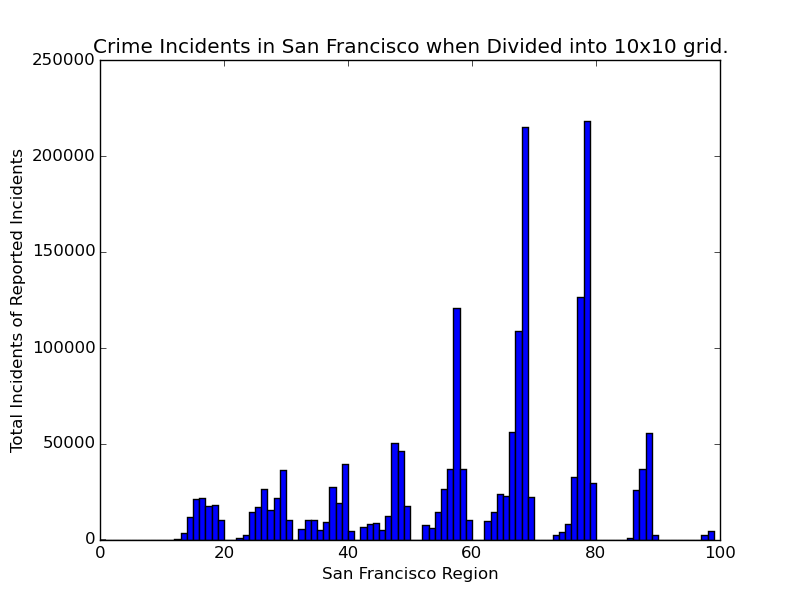
\includegraphics[scale=0.4]{sf_n10.png}
    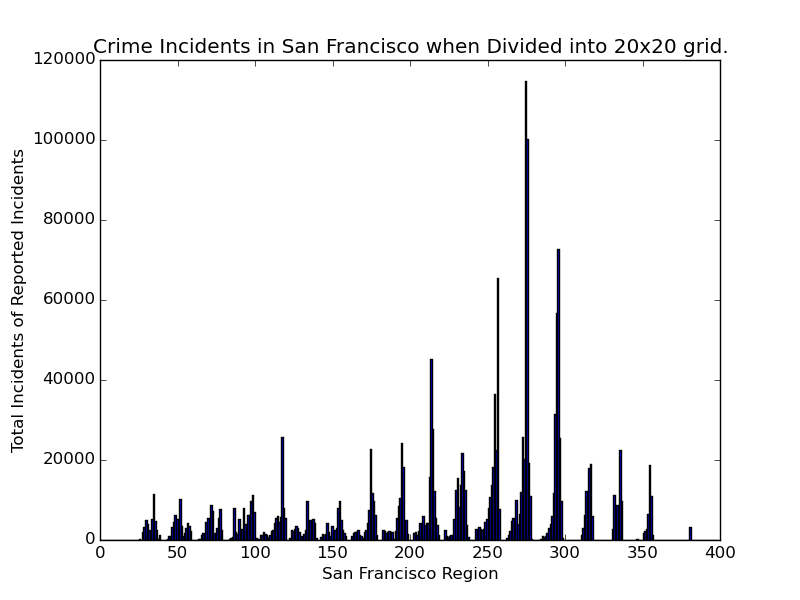
\includegraphics[scale=0.4]{sf_n20.png}
    \caption{Distribution of Crime Over Artificial Regions for the City of San Francisco}
    \label{fig:sf_100}
\end{figure}

We can explain the cyclic nature of the data extremely simply - most of the crime reported occurs in the central region of the city. The regions are numbered from the bottom right corner geographically, and continue westward until they fall outside the specified region, then moving upward to the next row. Therefore, we can imagine how moving in this fashion would lead to the above pattern in the data. Intuitively, however, we also have that most of the crime appears to occur in the northern region of San Francisco. \\

\section{Baseline Data}
% TODO: Baselines: Tables and/or figures. 

\subsection{Boston}
We now report some baselines results. We partition the city data into an $n \times n$ grid for $n \in [1, 5, 10, 25, 50, 75, 100]$. Then for each grid, we compute the number of crimes per month over the span of the entire dataset, approximately three years. We use a random $80\%$ of the data for training ridge regression (due to the few data points: ~36), and then compute the RMSE on the test set. We then average the RMSE over each square of the grid. Below we plot average RMSE over the entire grid vs $n$:\\

\begin{figure}[h!]
\centering
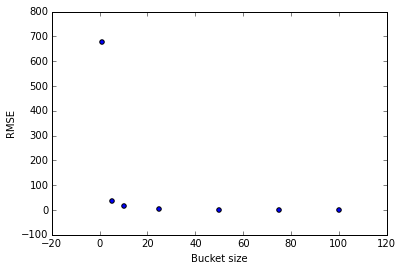
\includegraphics[scale=0.8]{boston_ridge.png}
\caption{RMSE vs Bucket Size $n$ for Boston}
\label{fig:bos_rmse}
\end{figure}

Figure \ref{fig:bos_rmse} reveals a pathology in this method: the RMSE decreases towards 0 as we increase $n$. We are creating smaller and smaller buckets, so that for large $n$, each bucket contains only a few data points while most contain 0. The Boston dataset in particular contains ~250,000 datapoints. Spread across the $100 \times 100$ buckets per timeframe and $36$ time frames means that by far most buckets have 0 crimes. Then the ridge regressor learns to predict 0 for most buckets, and gets a decent RMSE because even when there is a crime and it predicts 0, its error is small. Our hope is that Gaussian processes will not possess this pathology.

\begin{center}
\begin{tabular}{c|c}
 \textbf{n} & \textbf{avg RMSE} \\
 1 & 1254.35693616 \\
 5 & 36.8720866748 \\
 10 & 15.6527848706 \\
 25 & 3.55986509579 \\
 50 & 1.29333739045 \\
 75 & 0.72462817042 \\
 100 & 0.502453904579 \\
\end{tabular}
\end{center}

\subsection{San Francisco}
The process is similar to that used with Boston, though we show results only for $n \in [1,2,\cdots,10,20,\cdots,50]$. The testing data hold out is the most recent year. Data for San Francisco exists from early 2003, and we can see Figure \ref{fig:sf_100} for a distribution on the crime in the city.

\begin{figure}[h!]
\centering
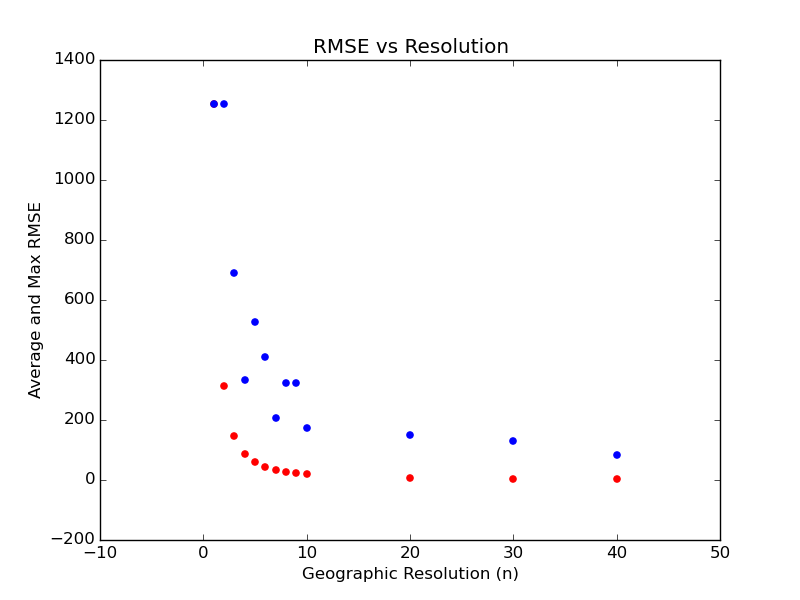
\includegraphics[scale=0.6]{sf_linear.png}
\caption{Average RMSE and Max RMSE on San Francisco Training Sample}
\label{fig:sf_rmse}
\end{figure}

\begin{center}
\begin{tabular}{c|c}
 \textbf{n} & \textbf{avg RMSE} \\
 1 & 676.610276256 \\
 5 & 57.9066942345 \\
 10 & 18.802226607 \\
 20 & 7.0541635899 \\ 
 30 & 4.0393275858 \\
 40 & 2.7812162903
\end{tabular}
\end{center}

\section{Future Work}
Our next step is fairly clear: begin exploring and understanding Gaussian processes. \\

One particular area of interests for us lies in exploring the city of Chicago. We've calculated baselines above for both Boston and San Francisco, so it shouldn't be difficult to replicate our work for the Chicago crime data. The only small issue we have is that Chicago has significantly more data, on the order of magnitude of gigabytes. We expect that in order to process this dataset, we will need to either partition it by year, which would limit our ability to train a model over the entire dataset, or move onto a cloud-platform such as AWS, Microsoft Azure, or a Harvard cluster. Any feedback regarding the feasibility of the latter would be greatly appreciated. \\

% Reference Section for Paper's we've READ ENTIRELY ONLY!
\bibliography{../references}{}
\bibliographystyle{plain}

\end{document}

